\documentclass[12pt]{article}
\usepackage{times}
\usepackage{amsmath}
\usepackage{a4}
\usepackage{graphicx}
\usepackage{hyperref}
\usepackage{fancyvrb}
%\setlength{\oddsidemargin}{-0.2in}
%\setlength{\evensidemargin}{-0.5in}
%\setlength{\textwidth}{7in}
%\newcommand{\beforeverb}{\footnotesize\begin{Verbatim}[frame=single]}
%\newcommand{\afterverb}{\end{Verbatim}\normalsize}
\begin{document}

\title{Numerical Analysis and Programming: Numpy Tutorial}
\author{Ying-Jer Kao}
\date{\today}

\maketitle
This tutorial is based on the the official \textit{tentative Numpy tutorial} (\url{http://www.scipy.org/Tentative_NumPy_Tutorial}), and you should always consult the official Numpy reference manual for information, see  \url{http://docs.scipy.org/doc/} for more details.

\section{Importing the NumPy module }
There are several ways to import NumPy. The standard approach is to use a simple import 
statement: 
\footnotesize
\begin{Verbatim}[frame=single]
>>> import numpy 
\end{Verbatim}
\normalsize
However, for large amounts of calls to NumPy functions, it can become tedious to write 
\texttt{numpy.X} over and over again. Instead, it is common to import under the briefer name \texttt{np}: 
\footnotesize
\begin{Verbatim}[frame=single]
>>> import numpy as np
\end{Verbatim}
\normalsize
This statement will allow us to access NumPy objects using \texttt{np.X} instead of \texttt{numpy.X}. It is 
also possible to import NumPy directly into the current namespace so that we don't have to use 
dot notation at all, but rather simply call the functions as if they were built-in: 
\footnotesize
\begin{Verbatim}[frame=single]
>>> from numpy import *
\end{Verbatim} 
\normalsize

However, this strategy is usually not recommended except for short interactive sessions because it 
removes some of the nice organization that modules provide. For the remainder of this tutorial, 
we will assume that the \texttt{import numpy as np} has been used. Notice \texttt{ipython} notebook automatically import  \texttt{numpy} and alias it as \texttt{np}.

\section{Basics}
NumPy's main object is the homogeneous multidimensional array. It is a table of elements (usually numbers), all of the same type, indexed by a tuple of positive integers. In Numpy dimensions are called \textit{axes} and the number of axes is \textit{rank}.
For example, the coordinates of a point in 3D space [1, 2, 1] is an array of rank 1, because it has one axis. That axis has a length of 3. In example pictured below, the array has rank 2 (it is 2-dimensional). The first dimension (axis) has a length of 2, the second dimension has a length of 3.
\footnotesize
\begin{Verbatim}[frame=single]
[[ 1., 0., 0.],
 [ 0., 1., 2.]]
 \end{Verbatim}
 \normalsize
 

Numpy's array class is called \texttt{ndarray}. It is also known by the alias \texttt{array}. The more important attributes of an ndarray object are:
\begin{itemize}
\item \textbf{\texttt{ndarray.ndim}} gives
the number of axes (dimensions) of the array. In the Python world, the number of dimensions is referred to as  \texttt{rank}.
\footnotesize
\begin{Verbatim}[frame=single]
>>> x = np.array( ((11,12,13), (21,22,23) ))
>>> x.ndim
2
\end{Verbatim}
\normalsize
\item \textbf{\texttt{ndarray.shape}} gives
the dimensions of the array. This is a tuple of integers indicating the size of the array in each dimension. For a matrix with \texttt{n} rows and \texttt{m} columns, shape will be \texttt{(n,m)}. The length of the shape tuple is therefore the rank, or number of dimensions, \texttt{ndim}.
\footnotesize
\begin{Verbatim}[frame=single]
>>> x = np.array(((7,3,0), (7,11,9), (15,3,7),(12,4,8)))
>>> x
array([[ 7,  3,  0],
       [ 7, 11,  9],
       [15,  3,  7],
       [12,  4,  8]])
>>> x.ndim
2
>>> x.shape
(4, 3)
>>> 
\end{Verbatim}
\normalsize
\item \textbf{\texttt{ndarray.size}} gives
the total number of elements of the array. This is equal to the product of the elements of shape.
\item \textbf{\texttt{ndarray.dtype}} gives
an object describing the type of the elements in the array. One can create or specify \texttt{dtype}'s using standard Python types. Additionally NumPy provides types of its own. \texttt{numpy.int32}, \texttt{numpy.int16}, and \texttt{numpy.float6} are some examples.
\item \textbf{\texttt{ndarray.itemsize}} gives
the size in bytes of each element of the array. For example, an array of elements of type \texttt{float64} has itemsize 8 (=64/8), while one of type complex32 has itemsize 4 (=32/8). 
\item \textbf{\texttt{ndarray.data}} gives
the buffer containing the actual elements of the array. Normally, we won't need to use this attribute because we will access the elements in an array using indexing facilities.
\end{itemize}


%The "shape" of an array denotes a tuple with the number of elements per axis (dimension) In our example in the picture, the shape is equal to \texttt{(6,3)}, i.e. we have 6 rows and 3 columns. 
%We can work with arrays like we are used to work with lists: 
%\footnotesize
%\begin{Verbatim}[frame=single]
%>>> x = np.array([42,47,11])
%>>> x[:2]
%array([42, 47])
%>>> x = np.array([42,47,11])
%>>> x[0]
%42
%>>> x[:2]
%array([42, 47])
%>>> x[1] = 49
%>>> x
%array([42, 49, 11])
%>>>
%\end{Verbatim}
%\normalsize



\section{Example}
\footnotesize
\begin{Verbatim}[frame=single]
>>>import numpy as np
>>> a = np.arange(15).reshape(3, 5)
>>> a
array([[ 0,  1,  2,  3,  4],
       [ 5,  6,  7,  8,  9],
       [10, 11, 12, 13, 14]])
>>> a.shape
(3, 5)
>>> a.ndim
2
>>> a.dtype.name
'int32'
>>> a.itemsize
4
>>> a.size
15
>>> type(a)
numpy.ndarray
>>> b = np.array([6, 7, 8])
>>> b
array([6, 7, 8])
>>> type(b)
numpy.ndarray
\end{Verbatim}
\normalsize

\section{Array Creation}
There are several ways to create arrays.
For example, you can create an array from a regular Python {list} or {tuple} using the  \texttt{array} function. The type of the resulting array is deduced from the type of the elements in the sequences.
\footnotesize
\begin{Verbatim}[frame=single]
>>> a = np.array( [2,3,4] )
>>> a
array([2, 3, 4])
>>> a.dtype
dtype('int32')
>>> b = np.array([1.2, 3.5, 5.1])
>>> b.dtype
dtype('float64')
\end{Verbatim}
\normalsize

A frequent error consists in calling \texttt{array} with multiple numeric arguments, rather than providing a \textit{single list of numbers} as an argument.
\footnotesize
\begin{Verbatim}[frame=single]
>>> a = np.array(1,2,3,4)    # WRONG
>>> a = np.array([1,2,3,4])  # RIGHT
\end{Verbatim}
\texttt{array} transforms sequences of sequences into two-dimensional arrays, sequences of sequences of sequences into three-dimensional arrays, and so on.
\footnotesize
\begin{Verbatim}[frame=single]
>>> b = np.array( [ (1.5,2,3), (4,5,6) ] )
>>> b
array([[ 1.5,  2. ,  3. ],
       [ 4. ,  5. ,  6. ]])
\end{Verbatim}
\normalsize

The type of the array can also be explicitly specified at creation time:
\footnotesize
\begin{Verbatim}[frame=single]
>>> c = array( [ [1,2], [3,4] ], dtype=complex )
>>> c
array([[ 1.+0.j,  2.+0.j],
       [ 3.+0.j,  4.+0.j]])
\end{Verbatim}
\normalsize

Often, the elements of an array are originally unknown, but its size is known. Hence, NumPy offers several functions to create arrays with initial placeholder content. These minimize the necessity of growing arrays, an expensive operation.
The function zeros creates an array full of zeros, the function ones creates an array full of ones, and the function empty creates an array whose initial content is random and depends on the state of the memory. By default, the \texttt{dtype} of the created array is \texttt{float64}.
\footnotesize
\begin{Verbatim}[frame=single]
>>> np.zeros( (3,4) )
array([[0.,  0.,  0.,  0.],
       [0.,  0.,  0.,  0.],
       [0.,  0.,  0.,  0.]])
>>> np.ones( (2,3,4), dtype=int16 )    
array([[[ 1, 1, 1, 1],
        [ 1, 1, 1, 1],
        [ 1, 1, 1, 1]],
       [[ 1, 1, 1, 1],
        [ 1, 1, 1, 1],
        [ 1, 1, 1, 1]]], dtype=int16)
>>> np.empty( (2,3) )
array([[ 3.73603959e-262, 6.02658058e-154, 6.55490914e-260],
       [ 5.30498948e-313, 3.14673309e-307, 1.00000000e+000]])
\end{Verbatim}
\normalsize

To create sequences of numbers, NumPy provides a function analogous to \texttt{range} that returns arrays instead of lists
\footnotesize
\begin{Verbatim}[frame=single]
>>> np.arange( 10, 30, 5 )
array([10, 15, 20, 25])
>>> np.arange( 0, 2, 0.3 )                
array([ 0., 0.3, 0.6, 0.9, 1.2, 1.5, 1.8])
\end{Verbatim}
\normalsize

When \texttt{arange} is used with floating point arguments, it is generally not possible to predict the number of elements obtained, due to the finite floating point precision. For this reason, it is usually better to use the function \texttt{linspace} that receives as an argument the number of elements that we want, instead of the step:
\footnotesize
\begin{Verbatim}[frame=single]
>>> np.linspace( 0, 2, 9 ) # 9 numbers from 0 to 2
array([ 0., 0.25, 0.5, 0.75, 1., 1.25, 1.5, 1.75, 2.])
>>> x = np.linspace( 0, 2*np.pi, 100 ) 
>>> f = np.sin(x)
\end{Verbatim}
\normalsize

\section{Basic Operations}
Arithmetic operators on arrays apply elementwise. A new array is created and filled with the result.
\footnotesize
\begin{Verbatim}[frame=single]
>>> a = np.array( [20,30,40,50] )
>>> b = np.arange( 4 )
>>> b
array([0, 1, 2, 3])
>>> c = a-b
>>> c
array([20, 29, 38, 47])
>>> b**2
array([0, 1, 4, 9])
>>> 10*np.sin(a)
array([ 9.12945251, -9.88031624,  7.4511316 , -2.62374854])
>>> a<35
array([True, True, False, False], dtype=bool)
\end{Verbatim}
\normalsize
Unlike in many matrix languages, the product operator * operates \textit{elementwise} in NumPy arrays. The matrix product can be performed using the \texttt{dot} function or creating matrix objects.
\footnotesize
\begin{Verbatim}[frame=single]
>>> A = np.array( [[1,1],
...             [0,1]] )
>>> B = np.array( [[2,0],
...             [3,4]] )
>>> A*B # elementwise product
array([[2, 0],
       [0, 4]])
>>> dot(A,B) # matrix product
array([[5, 4],
       [3, 4]])
 \end{Verbatim}
\normalsize
      
Some operations, such as \texttt{+=} and \texttt{*=}, act in place to modify an existing array rather than create a new one.
\footnotesize
\begin{Verbatim}[frame=single]
>>> a = np.ones((2,3), dtype=int)
>>> b = np.random.random((2,3))
>>> a *= 3
>>> a
array([[3, 3, 3],
       [3, 3, 3]])
>>> b += a
>>> b
array([[ 3.69092703,  3.8324276 ,  3.0114541 ],
       [ 3.18679111,  3.3039349 ,  3.37600289]])
>>> a += b  # b is converted to integer type
>>> a
array([[6, 6, 6],
       [6, 6, 6]])
\end{Verbatim}
\normalsize

When operating with arrays of different types, the type of the resulting array corresponds to the more general or precise one (a behavior known as \textit{upcasting}).
\footnotesize
\begin{Verbatim}[frame=single]
>>> a = np.ones(3, dtype=int32)
>>> b = np.linspace(0,pi,3)
>>> b.dtype.name
'float64'
>>> c = a+b
>>> c
array([ 1.,  2.57079633,  4.14159265])
>>> c.dtype.name
'float64'
>>> d = exp(c*1j)
>>> d
array([ 0.54030231+0.84147098j, -0.84147098+0.54030231j,
       -0.54030231-0.84147098j])
>>> d.dtype.name
'complex128'
\end{Verbatim}
\normalsize

\section{Universal Functions}
NumPy provides familiar mathematical functions such as \texttt{sin}, \texttt{cos}, and \texttt{exp}, etc. In NumPy, these are called "universal functions"(ufunc). Within NumPy, these functions operate \textit{elementwise} on an array, producing an array as output.
\footnotesize
\begin{Verbatim}[frame=single]
>>> B = np.arange(3)
>>> B
array([0, 1, 2])
>>> np.exp(B)
array([ 1.,  2.71828183,  7.3890561 ])
>>> np.sqrt(B)
array([ 0.,  1.,  1.41421356])
>>> C = np.array([2., -1., 4.])
>>> np.add(B, C)
array([ 2.,  0.,  6.])
\end{Verbatim}
\normalsize
The items in an array can be summed or multiplied: 
\footnotesize
\begin{Verbatim}[frame=single]
>>> a = np.array([2, 4, 3], float) 
>>> a.sum() 
9.0 
>>> a.prod() 
24.0 
\end{Verbatim}
\normalsize
In this example, member functions of the arrays were used. Alternatively, standalone functions 
in the NumPy module can be accessed: 
\footnotesize
\begin{Verbatim}[frame=single]
>>> np.sum(a) 
9.0 
>>> np.prod(a) 
24.0 
\end{Verbatim}
\normalsize
For most of the routines described below, both standalone and member functions are available. 
A number of routines enable computation of statistical quantities in array datasets, such as the 
mean (average), variance, and standard deviation: 
\footnotesize
\begin{Verbatim}[frame=single]
>>> a = np.array([2, 1, 9], float) 
>>> a.mean() 
4.0 
>>> a.var() 
12.666666666666666 
>>> a.std() 
3.5590260840104371
\end{Verbatim}
\normalsize
It's also possible to find the minimum and maximum element values: 
\footnotesize
\begin{Verbatim}[frame=single]
>>> a = np.array([2, 1, 9], float) 
>>> a.min() 
1.0 
>>> a.max() 
9.0 
\end{Verbatim}
\normalsize
The \texttt{argmin} and \texttt{argmax} functions return the array indices of the minimum and maximum 
values: 
\footnotesize
\begin{Verbatim}[frame=single]
>>> a = np.array([2, 1, 9], float) 
>>> a.argmin()
1
>>> a.argmax()
2
\end{Verbatim}
\normalsize
For multidimensional arrays, each of the functions thus far described can take an optional argument axis that will perform an operation along only the specified axis, placing the results in a return array:
\footnotesize
\begin{Verbatim}[frame=single]
>>> a = np.array([[0, 2], [3, -1], [3, 5]], float) 
>>> a.mean(axis=0)
array([ 2., 2.])
>>> a.mean(axis=1)
array([ 1.,  1.,  4.])
>>> a.min(axis=1)
array([ 0., -1.,  3.])
>>> a.max(axis=0)
array([ 3., 5.]) 
\end{Verbatim}
\normalsize
\section{Array mathematics }
When standard mathematical operations are used with arrays, they are applied on an \textit{element-wise} basis. This means that the arrays should be the same size during addition, subtraction, etc.:
\footnotesize
\begin{Verbatim}[frame=single] 
>>> a = np.array([1,2,3], float) 
>>> b = np.array([5,2,6], float) 
>>> a + b 
array([6., 4., 9.]) 
>>> a – b 
array([-4., 0., -3.]) 
>>> a * b 
array([5., 4., 18.]) 
>>> b / a 
array([5., 1., 2.]) 
>>> a % b 
array([1., 0., 3.]) 
>>> b**a 
array([5., 4., 216.]) 
\end{Verbatim}
\normalsize
For two-dimensional arrays, multiplication remains elementwise and does not correspond to 
matrix multiplication. There are special functions for matrix math that we will cover later. 
\footnotesize
\begin{Verbatim}[frame=single]
>>> a = np.array([[1,2], [3,4]], float) 
>>> b = np.array([[2,0], [1,3]], float) 
>>> a * b 
array([[2., 0.], [3., 12.]]) 
\end{Verbatim}
\normalsize
Errors are thrown if arrays do not match in size:
\footnotesize
\begin{Verbatim}[frame=single]
>>> a = np.array([1,2,3], float) 
>>> b = np.array([4,5], float) 
>>> a + b
Traceback (most recent call last): 
  File "<stdin>", line 1, in <module> 
ValueError: shape mismatch: 
objects cannot be broadcast to a single shape
\end{Verbatim}
\normalsize
\section{Vector and matrix mathematics }
NumPy provides many functions for performing standard vector and matrix multiplication 
routines. To perform a dot product, 
\footnotesize
\begin{Verbatim}[frame=single]
>>> a = np.array([1, 2, 3], float) 
>>> b = np.array([0, 1, 1], float) 
>>> np.dot(a, b) 
5.0 
\end{Verbatim}
\normalsize
The dot function also generalizes to matrix multiplication: 
\footnotesize
\begin{Verbatim}[frame=single]
>>> a = np.array([[0, 1], [2, 3]], float) 
>>> b = np.array([2, 3], float) 
>>> c = np.array([[1, 1], [4, 0]], float) 
>>> a 
array([[ 0., 1.], 
 [ 2., 3.]]) 
>>> np.dot(b, a) 
array([ 6., 11.]) 
>>> np.dot(a, b) 
array([ 3., 13.]) 
>>> np.dot(a, c) 
array([[ 4., 0.], 
 [ 14., 2.]]) 
>>> np.dot(c, a) 
array([[ 2., 4.], 
 [ 0., 4.]]) 
\end{Verbatim}
\normalsize
It is also possible to generate inner, outer, and cross products of matrices and vectors. For 
vectors, note that the inner product is equivalent to the dot product: 
\footnotesize
\begin{Verbatim}[frame=single]
>>> a = np.array([1, 4, 0], float) 
>>> b = np.array([2, 2, 1], float) 
>>> np.outer(a, b) 
array([[ 2., 2., 1.], 
 [ 8., 8., 4.], 
 [ 0., 0., 0.]]) 
>>> np.inner(a, b) 
10.0 
>>> np.cross(a, b) 
array([ 4., -1., -6.]) 
\end{Verbatim}
\normalsize
For a high-dimensional tensors, the function \texttt{tensordot} computes tensor dot product along specified axes.
\footnotesize
\begin{Verbatim}[frame=single]
>>>((2,4,3)))
>>> a=np.array(np.random.random((2,4,3)))
>>> a
array([[[ 0.52915858,  0.2623554 ,  0.57765439],
        [ 0.50031623,  0.18099146,  0.19391296],
        [ 0.56486312,  0.20455544,  0.15219032],
        [ 0.96975173,  0.0520726 ,  0.5611672 ]],

       [[ 0.95568698,  0.60541739,  0.657405  ],
        [ 0.21022514,  0.27462493,  0.32806541],
        [ 0.80856084,  0.06451977,  0.33994045],
        [ 0.46833801,  0.35243041,  0.83470196]]])
>>>>>> b=np.array(np.random.random((4,3,2)))
>>> b
array([[[ 0.87176381,  0.68883495],
        [ 0.16451053,  0.8020721 ],
        [ 0.82210924,  0.15417885]],

       [[ 0.01163689,  0.67328002],
        [ 0.61299208,  0.61937904],
        [ 0.91849722,  0.05603531]],

       [[ 0.66886977,  0.20655257],
        [ 0.06674962,  0.33113124],
        [ 0.05115619,  0.75813028]],

       [[ 0.50889226,  0.44853399],
        [ 0.30247792,  0.63194832],
        [ 0.83564744,  0.98830335]]])
>>>np.tensordot(a,b, axes=2)
array([[ 2.65168075,  2.44608012],
       [ 3.55027721,  3.27909354]])
>>> a = np.arange(60.).reshape(3,4,5)
>>> b = np.arange(24.).reshape(4,3,2)
>>> c = np.tensordot(a,b, axes=([1,0],[0,1]))
>>> c.shape
(5, 2)
>>> c
array([[ 4400.,  4730.],
       [ 4532.,  4874.],
       [ 4664.,  5018.],
       [ 4796.,  5162.],
       [ 4928.,  5306.]])
\end{Verbatim}
\normalsize

NumPy also provides a number of built-in routines for linear algebra calculations. These can 
be found in the sub-module \texttt{linalg}. Among these are routines for dealing with matrices and 
their inverses. The determinant of a matrix can be found: 
\footnotesize
\begin{Verbatim}[frame=single]
>>> a = np.array([[4, 2, 0], [9, 3, 7], [1, 2, 1]], float) 
>>> a 
array([[ 4., 2., 0.], 
 [ 9., 3., 7.], 
 [ 1., 2., 1.]]) 
>>> np.linalg.det(a) 
-53.999999999999993 
\end{Verbatim}
\normalsize
One can find the eigenvalues and eigenvectors of a matrix: 
\footnotesize
\begin{Verbatim}[frame=single]
>>> vals, vecs = np.linalg.eig(a) 
>>> vals 
array([ 9. , 2.44948974, -2.44948974]) 
>>> vecs 
array([[-0.3538921 , -0.56786837, 0.27843404], 
 [-0.88473024, 0.44024287, -0.89787873], 
 [-0.30333608, 0.69549388, 0.34101066]]) 
\end{Verbatim}
\normalsize
The inverse of a matrix can be found: 
\footnotesize
\begin{Verbatim}[frame=single]
>>> b = np.linalg.inv(a) 
>>> b 
array([[ 0.14814815, 0.07407407, -0.25925926], 
 [ 0.2037037 , -0.14814815, 0.51851852], 
 [-0.27777778, 0.11111111, 0.11111111]]) 
>>> np.dot(a, b) 
array([[ 1.00000000e+00, 5.55111512e-17, 2.22044605e-16], 
 [ 0.00000000e+00, 1.00000000e+00, 5.55111512e-16], 
 [ 1.11022302e-16, 0.00000000e+00, 1.00000000e+00]])
\end{Verbatim}
\normalsize
Singular value decomposition (analogous to diagonalization of a nonsquare matrix) can also be 
performed: 
\footnotesize
\begin{Verbatim}[frame=single]
>>> a = np.array([[1, 3, 4], [5, 2, 3]], float) 
>>> U, s, Vh = np.linalg.svd(a) 
>>> U 
array([[-0.6113829 , -0.79133492], 
 [-0.79133492, 0.6113829 ]]) 
>>> s 
array([ 7.46791327, 2.86884495]) 
>>> Vh 
array([[-0.61169129, -0.45753324, -0.64536587], 
 [ 0.78971838, -0.40129005, -0.46401635], 
 [-0.046676 , -0.79349205, 0.60678804]]) 
\end{Verbatim}
\normalsize
\section{Indexing, Slicing and Iterating}
\textbf{One-dimensional arrays} can be indexed, sliced and iterated over, much like lists and other Python sequences.
\footnotesize
\begin{Verbatim}[frame=single]
>>> a = np.arange(10)**3
>>> a
array([  0,   1,   8,  27,  64, 125, 216, 343, 512, 729])
>>> a[2]
8
>>> a[2:5]
array([ 8, 27, 64])
>>> a[:6:2] = -1000    
>>> a
array([-1000, 1, -1000, 27, -1000, 125, 216, 343, 512, 729])
>>> a[ : :-1]   
array([  729, 512, 343, 216, 125, -1000, 27, -1000, 1, -1000])
>>> for i in a:
...         print i**(1/3.),
...
nan 1.0 nan 3.0 nan 5.0 6.0 7.0 8.0 9.0
\end{Verbatim}
\normalsize
\textbf{Multidimensional arrays} can have one index per axis. These indices are given in a tuple separated by commas:
\footnotesize
\begin{Verbatim}[frame=single]
>>> def f(x,y):
...         return 10*x+y
...
>>> b = fromfunction(f,(5,4),dtype=int)
>>> b
array([[ 0,  1,  2,  3],
       [10, 11, 12, 13],
       [20, 21, 22, 23],
       [30, 31, 32, 33],
       [40, 41, 42, 43]])
>>> b[2,3]
23
>>> b[0:5, 1]                       
array([ 1, 11, 21, 31, 41])
>>> b[ : ,1]                        
array([ 1, 11, 21, 31, 41])
>>> b[1:3, : ]                   
array([[10, 11, 12, 13],
       [20, 21, 22, 23]])
\end{Verbatim}
\normalsize
\begin{figure}[ht]
\centerline{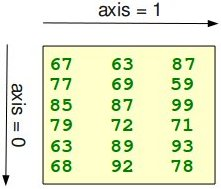
\includegraphics[width=0.4\textwidth]{axis1.jpeg}\hspace{0.2in}
\includegraphics[width=0.4\textwidth]{axis.jpeg}}
\caption{Examples of rank-2 and -3 arrays.}
\end{figure}


When fewer indices are provided than the number of axes, the missing indices are considered complete slices:
\footnotesize
\begin{Verbatim}[frame=single]
>>> b[-1]   
array([40, 41, 42, 43])
\end{Verbatim}
\normalsize
The expression within brackets in \texttt{b[i]} is treated as an \texttt{i} followed by as many instances of \texttt{:} as needed to represent the remaining axes. NumPy also allows you to write this using dots as \texttt{b[i,...]}.
The dots (\texttt{...}) represent as many colons as needed to produce a complete indexing tuple. For example, if {\tt x} is a rank 5 array (i.e., it has 5 axes), then
\texttt{x[1,2,...]} is equivalent to \texttt{x[1,2,:,:,:]},
\texttt{x[...,3]} to \texttt{x[:,:,:,:,3]} and
\texttt{x[4,...,5,:]} to \texttt{x[4,:,:,5,:]}.
\footnotesize
\begin{Verbatim}[frame=single]
>>> c = array( [ [[  0,  1,  2], 
...               [ 10, 12, 13]],
...              [[100,101,102],
...               [110,112,113]] ] )
>>> c.shape
(2, 2, 3)
>>> c[1,...]  # same as c[1,:,:] or c[1]
array([[100, 101, 102],
       [110, 112, 113]])
>>> c[...,2]  # same as c[:,:,2]
array([[  2,  13],
       [102, 113]])
\end{Verbatim}
\normalsize
Iterating over multidimensional arrays is done with respect to the first axis:
\footnotesize
\begin{Verbatim}[frame=single]
>>> for row in b:
...         print row
...
[0 1 2 3]
[10 11 12 13]
[20 21 22 23]
[30 31 32 33]
[40 41 42 43]
\end{Verbatim}
\normalsize
However, if one wants to perform an operation on each element in the array, one can use the flat attribute which is an iterator over all the elements of the array:
\footnotesize
\begin{Verbatim}[frame=single]
>>> for element in b.flat:
...         print element,
...
0 1 2 3 10 11 12 13 20 21 22 23 30 31 32 33 40 41 42 43
\end{Verbatim}
\normalsize

\section{Shape Manipulation}
\subsection{Changing the shape of an array}
An array has a shape given by the number of elements along each axis:
\footnotesize
\begin{Verbatim}[frame=single]
>>> a = floor(10*random.random((3,4)))
>>> a
array([[ 7.,  5.,  9.,  3.],
       [ 7.,  2.,  7.,  8.],
       [ 6.,  8.,  3.,  2.]])
>>> a.shape
(3, 4)
\end{Verbatim}
\normalsize
The shape of an array can be changed with various commands:
\footnotesize
\begin{Verbatim}[frame=single]
>>> a.ravel() # flatten the array
array([ 7., 5., 9., 3., 7., 2., 7., 8., 6., 8., 3., 2.])
>>> a.shape = (6, 2)
>>> a.transpose()
array([[ 7., 9., 7., 7., 6., 3.],
       [ 5., 3., 2., 8., 8., 2.]])
\end{Verbatim}
\normalsize

The order of the elements in the array resulting from \texttt{ravel()} is normally "C-style", that is, the rightmost index "changes the fastest", so the element after \texttt{a[0,0]} is \texttt{a[0,1]}. If the array is reshaped to some other shape, again the array is treated as "C-style".  The functions \texttt{ravel()} and \texttt{reshape()} can also be instructed, using an optional argument, to use FORTRAN-style arrays, in which the leftmost index changes the fastest.
\begin{figure}[ht]
\centerline{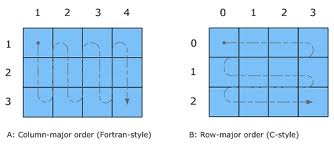
\includegraphics[width=0.8\textwidth]{memory.jpeg}}
\caption{Memory layout of a FORTRAN-style  and a C-style array.} 
\end{figure}

The \texttt{reshape} function returns its argument with a modified shape, whereas the \texttt{resize} method modifies the array itself:
\footnotesize
\begin{Verbatim}[frame=single]
>>> a
array([[ 7., 5.],
       [ 9., 3.],
       [ 7., 2.],
       [ 7., 8.],
       [ 6., 8.],
       [ 3., 2.]])
>>> a.resize((2,6))
>>> a
array([[ 7., 5., 9., 3., 7., 2.],
       [ 7., 8., 6., 8., 3., 2.]])
\end{Verbatim}
\normalsize
If a dimension is given as -1 in a reshaping operation, the other dimensions are automatically calculated:
\footnotesize
\begin{Verbatim}[frame=single]
>>> a.reshape(3,-1)
array([[ 7., 5., 9., 3.],
       [ 7., 2., 7., 8.],
       [ 6., 8., 3., 2.]])
\end{Verbatim}
\normalsize

\subsection{Stacking together different arrays}
Several arrays can be stacked together along different axes:
\footnotesize
\begin{Verbatim}[frame=single]
>>> a = np.floor(10*np.random.random((2,2)))
>>> a
array([[ 1., 1.],
       [ 5., 8.]])
>>> b = np.floor(10*np.random.random((2,2)))
>>> b
array([[ 3., 3.],
       [ 6., 0.]])
>>> np.vstack((a,b))
array([[ 1., 1.],
       [ 5., 8.],
       [ 3., 3.],
       [ 6., 0.]])
>>> np.hstack((a,b))
array([[ 1., 1., 3., 3.],
       [ 5., 8., 6., 0.]])
\end{Verbatim}
\normalsize
The function \verb!column_stack! stacks 1D arrays as columns into a 2D array. It is equivalent to \texttt{vstack} only for 1D arrays:
\footnotesize
\begin{Verbatim}[frame=single]
>>> column_stack((a,b))   # With 2D arrays
array([[ 1., 1., 3., 3.],
       [ 5., 8., 6., 0.]])
>>> a=np.array([4.,2.])
>>> b=np.array([2.,8.])
>>> a[:,np.newaxis]  
array([[ 4.],
       [ 2.]])
>>> column_stack((a[:,np.newaxis],b[:,np.newaxis]))
array([[ 4., 2.],
       [ 2., 8.]])
>>> vstack((a[:,np.newaxis],b[:,np.newaxis])) 
array([[ 4.],
       [ 2.],
       [ 2.],
       [ 8.]])
\end{Verbatim}
\normalsize

\subsection{Splitting one array into several smaller ones}
Using \texttt{hsplit}, you can split an array along its horizontal axis, either by specifying the number of equally shaped arrays to return, or by specifying the columns after which the division should occur:
\footnotesize
\begin{Verbatim}[frame=single]
>>> a = floor(10*np.random.random((2,12)))
>>> a
array([[ 8., 8., 3., 9., 0., 4., 3., 0., 0., 6., 4., 4.],
       [ 0., 3., 2., 9., 6., 0., 4., 5., 7., 5., 1., 4.]])
>>> np.hsplit(a,3)   # Split a into 3
[array([[ 8., 8., 3., 9.],
       [ 0., 3., 2., 9.]]), array([[ 0., 4., 3., 0.],
       [ 6., 0., 4., 5.]]), array([[ 0., 6., 4., 4.],
       [ 7., 5., 1., 4.]])]
>>> np.hsplit(a,(3,4))   
[array([[ 8., 8., 3.],
       [ 0., 3., 2.]]), array([[ 9.],
       [ 9.]]), array([[ 0., 4., 3., 0., 0., 6., 4., 4.],
       [ 6., 0., 4., 5., 7., 5., 1., 4.]])]
\end{Verbatim}
\normalsize
\texttt{vsplit} splits along the vertical axis, and array split allows one to specify along which axis to split.

\section{Copies and Views}
When operating and manipulating arrays, their data is sometimes copied into a new array and sometimes not. This is often a source of confusion for beginners. There are three cases:
\subsection{No Copy at All}
Simple assignments make no copy of array objects or of their data.
\footnotesize
\begin{Verbatim}[frame=single]
>>> a = np.arange(12)
>>> b = a            # no new object is created
>>> b is a           
True
>>> b.shape = 3,4    
>>> a.shape
(3, 4)
\end{Verbatim}
\normalsize
Python passes mutable objects as \textit{references}, so function calls make no copy.
\footnotesize
\begin{Verbatim}[frame=single]
>>> def f(x):
...     print id(x)
...
>>> id(a)     # id is a unique identifier of an object
148293216
>>> f(a)
148293216
\end{Verbatim}
\normalsize
\subsection{View or Shallow Copy}
Different array objects can share the same data. The \texttt{view} method creates a new array object that looks at the same data.
\footnotesize
\begin{Verbatim}[frame=single]
>>> c = a.view()
>>> c is a
False
>>> c.base is a                      
True
>>> c.flags.owndata
False
>>>
>>> c.shape = 2,6                      
>>> a.shape
(3, 4)
>>> c[0,4] = 1234                   
>>> a
array([[   0,    1,    2,    3],
       [1234,    5,    6,    7],
       [   8,    9,   10,   11]])
\end{Verbatim}
\normalsize
Slicing an array returns a view of it:
\footnotesize
\begin{Verbatim}[frame=single]
>>> s = a[ : , 1:3]     
>>> s[:] = 10           
>>> a
array([[   0,   10,   10,    3],
       [1234,   10,   10,    7],
       [   8,   10,   10,   11]])
\end{Verbatim}
\normalsize
\subsection{Deep Copy}
The copy method makes a complete copy of the array and its data.
\footnotesize
\begin{Verbatim}[frame=single]
>>> d = a.copy()     
>>> d is a
False
>>> d.base is a                 
False
>>> d[0,0] = 9999
>>> a
array([[   0,   10,   10,    3],
       [1234,   10,   10,    7],
       [   8,   10,   10,   11]])
\end{Verbatim}
\normalsize

\end{document}	
